%
% $Id: SANDtemplate.tex,v 1.3 2007-12-13 21:27:14 rolf Exp $
% A template to build SAND reports. See the examples for more details and
% formatting suggestions. A command reference is available at
% http://www.cs.sandia.gov/~rolf/SANDreport
%
\documentclass[12pt]{SANDreport}


% ---------------------------------------------------------------------------- %
% Set the title, author, and date
%
\title{Data Co-Processing for Extreme Scale Analysis Level II ASC Milestone
  (4745)}
% Formatting for a line with an Author's Name
\newcommand*{\anline}[1]{#1 \\[-1ex]}
% Formatting for a line of an Author's Address
\newcommand*{\aaline}[1]{{\small #1} \\[-1ex]}
\author{
  \anline{David Rogers}
  \aaline{Scalable Analysis and Visualization}
  \aaline{Sandia National Laboratories}
  \aaline{P.O. Box 5800 MS 1326}
  \aaline{Albuquerque, NM 87185-1326}
  \aaline{dhroger@sandia.gov}
  \and
  \anline{Kenneth Moreland}
  \aaline{Scalable Analysis and Visualization}
  \aaline{Sandia National Laboratories}
  \aaline{P.O. Box 5800 MS 1326}
  \aaline{Albuquerque, NM 87185-1326}
  \aaline{kmorel@sandia.gov}
  \and
  \anline{Ron Oldfield}
  \aaline{Scalable System Software}
  \aaline{Sandia National Laboratories}
  \aaline{P.O. Box 5800 MS 1319}
  \aaline{Albuquerque, NM 87185-1319}
  \aaline{raoldfi@sandia.gov}
  \and
  \anline{Nathan Fabian}
  \aaline{Scalable Analysis and Visualization}
  \aaline{Sandia National Laboratories}
  \aaline{P.O. Box 5800 MS 1323}
  \aaline{Albuquerque, NM 87185-1323}
  \aaline{ndfabian@sandia.gov}
}
\date{}             % Leave this here but empty


% ---------------------------------------------------------------------------- %
% These are mandatory
%
\SANDnum{SAND2013-XXXX} % e.g. \SANDnum{SAND2006-0420}
\SANDprintDate{March 2013} % Month, year
\SANDauthor{David Rogers, Kenneth Moreland, Ron Oldfield, and Nathan Fabian}


% ---------------------------------------------------------------------------- %
% These are optional
%
%\SANDrePrintDate{}     % May be repeated for successive printings
%\SANDsupersed{}{}      % {Old SAND number}{Old date}


% ---------------------------------------------------------------------------- %
% Build your markings. See example files and SAND Report Guide
%
    %\SANDreleaseType{}
    %\SANDmarkTopBottomCoverBackTitle{}
    %\SANDmarkBottomCover{}
    %\SANDmarkTopBottomCoverTitle{}
    %\SANDmarkTop{}
    %\SANDmarkBottom{}
    %\SANDmarkTopBottom{}
    %\SANDmarkCover{}
    %\SANDmarkCoverTitle{}


\usepackage{booktabs}
\usepackage{cite}
\usepackage{graphicx}
\usepackage{placeins}
\usepackage{subfig}
\usepackage{xspace}

\usepackage[hidelinks]{hyperref}

\usepackage{color}
\definecolor{yellow}{rgb}{1,1,0}
\definecolor{black}{rgb}{0,0,0}
\definecolor{ltcyan}{rgb}{.75,1,1}
\definecolor{red}{rgb}{1,0,0}
\definecolor{gray}{rgb}{.6,.6,.6}
\definecolor{darkred}{rgb}{0.5,0,0}
\definecolor{darkgreen}{rgb}{0,0.5,0}

% Cite commands I use to abstract away the different ways to reference an
% entry in the bibliography (superscripts, numbers, dates, or author
% abbreviations).  \scite is a short cite that is used immediately after
% when the authors are mentioned.  \lcite is a full citation that is used
% anywhere.  Both should be used right next to the text being cited without
% any spacing.
\newcommand*{\lcite}[1]{~\cite{#1}}
\newcommand*{\scite}[1]{~\cite{#1}}

% Convenience commands to save time typing and to ensure that we have
% consistent use and typography.
\newcommand{\vda}{visualization and data analysis\xspace}
\newcommand{\Insitu}{\emph{In situ}\xspace}
\newcommand{\insitu}{\emph{in situ}\xspace}
\newcommand{\intransit}{\emph{in transit}\xspace}
\newcommand{\Intransit}{\emph{In transit}\xspace}
\newcommand{\etal}{et al.}

\newcommand*{\keyterm}[1]{\textbf{#1}}

% This is a command I use to make notes to myself or other authors in the
% document.  The text is noticeable in the document and easy to search for
% in the tex file.  It is also easy to turn them all off by simply
% replacing the command with one that does nothing.
%\newcommand{\fix}[1]{{\color{red}\textsc{[#1]}}}
\newcommand{\fix}[1]{}

% Hyphenation of words that do not follow standard English rules.
\hyphenation{Para-View}

% Avoid putting figures on their own page.
\renewcommand{\textfraction}{0.05}
\renewcommand{\topfraction}{0.95}
\renewcommand{\bottomfraction}{0.95}

% Make sure this is big enough so that only big figures end up on their own
% page but small enough so that if a figure does have to be on its own
% page, it won't push everything to the bottom because it's not big enough
% to have its own page.
\renewcommand{\floatpagefraction}{.75}

% ---------------------------------------------------------------------------- %
% Start the document
%
\begin{document}

\sloppy

\maketitle

% ------------------------------------------------------------------------ %
% An Abstract is required for SAND reports
%
\begin{abstract}

\fix{Dave and/or Ken}

\end{abstract}



%% % ------------------------------------------------------------------------ %
%% % An Acknowledgment section is optional but important
%% %
%% \clearpage
%% \section*{Acknowledgment}


% ------------------------------------------------------------------------ %
% The table of contents and list of figures and tables
%
\cleardoublepage            % TOC needs to start on an odd page
\tableofcontents
\listoffigures
\listoftables


%% % ---------------------------------------------------------------------- %
%% % An optional preface or Foreword
%% \clearpage
%% \section*{Preface}
%% \addcontentsline{toc}{section}{Preface}


% ---------------------------------------------------------------------- %
% An optional executive summary
\clearpage
\section*{Executive Summary}
\addcontentsline{toc}{section}{Executive Summary}

Milestone 4745 Data Co-Processing for Extreme Scale Analysis was successfully completed on time, and demonstrated against the letter and spirit of the stated Milestone.

\begin{quote}
\begin{em}
SNL will engineer, test and evaluate customer-driven operations on a large-scale data created by a running simulation.  The data operations will be performed by both in-situ and in-transit solutions
\end{em}
\end{quote}

Both in-situ (Catalyst) and in-transit (Nessie) analysis capabilities were engineered, tested and evaluated by coupling with CTH running a fragmentation problem, provided by a Sandia analyst, at scales up to 64k cores on Cielo.

Though simply stated, this represented the bulk of the development work on the Milestone, requiring that the in-situ and in-transit capabilities by developed, engineered and tested at scale. 

\begin{quote}
\begin{em}
The resulting performance data published and made available to the ASC community.
\end{em}
\end{quote}

Proof:  The full results have been published in a SAND report, and is available to anyone.




%% % ---------------------------------------------------------------------- %
%% % An optional glossary. We don't want it to be numbered
%% \clearpage
%% \section*{Nomenclature}
%% \addcontentsline{toc}{section}{Nomenclature}
%% \begin{description}
%% \item[Term 1]
%%   Description
%% \item[Term 2]
%%   Description
%% \item[Term 3]
%%   Description
%% \end{description}


% ---------------------------------------------------------------------- %
% This is where the body of the report begins; usually with an Introduction
%
\SANDmain           % Start the main part of the report

\section{Official Milestone}
\label{sec:OfficialMilestone}

\fix{A copy of the official wording of the milestone.}


%% \section{Background}
\label{sec:Background}

\fix{Not sure if the following really need to be subsections or just
  paragraphs in a narrative.}

\subsection{Simulation Context}

\subsection{Current Post-Processing Pipelines}

\subsection{I/O Bottleneck}

\subsection{Motivation}

\fix{Some motivating discussion can be found in this workshop
  report:~\cite{ScientificDiscoveryExascale2011}.}

\subsubsection{Catalyst}

\subsubsection{Nessie}


%% \section{Scope}
\label{sec:Scope}

\subsection{State of the Art}

When this Milestone was designed, there were three types of activities that addressed large scale data analysis: post-processing, code-specific in-situ solutions, and communication frameworks concerned with data movement.

Specialized solutions are specific instantiations of in-situ processing tuned for a particular code.  Examples include CTH's \fix{blar} and the \fix{other blar that Kwan Liu is developing with Jackie Chan}.  These are highly efficient in-situ analysis codes developed in tandem with a specific code, and represent the pathway to the most efficient in-situ solution, tuned for the data structures, the memory/compute time trade-offs and analysis needs of a specific customer in a specific domain.  As such, we expect that specialized solutions will always offer the most compact, optimized in-situ processing for the codes they were designed for.  However, applying these in-situ codes to other domains and codes requires an investment in engineering (they cannot always be easily abstracted from the target code), a trade-off in flexibility (they are often designed to achieve a specific analysis or visualization task, often one that lends itself to optimization at large scale), and a trade-off in community support and engagement.

Another option for large scale in-situ analysis is to create a capability that is intended to support a large range of data types, analysis operations and visualization modes.  A generalized engineering solution would be more flexible, but perhaps less efficient than one tuned for a specific code.  This type of library would provide analysis capabilities for a range of problems, providing a method of prototyping and iterating on many types of analysis.  Valuable or common analysis operations can then be optimized as needed for specific codes.  This is the option that is at the core of our Milestone.

The value of this contribution is to promote the investigation of a larger trade-off space, in which memory, compute time, analysis type, and storage can all be traded more flexibly to achieve a required analytics end.  By building a robust, cross-platform capability for large scale in-situ analysis, we hope to build a community that exercises different options in the trade-off space, allowing analysts and scientists the capability to explore the impact of different combinations of memory, processing time, energy, storage, analysis algorithms to achieve their results.  In particular, as we continue towards larger, ever diverse computation platforms, it is beneficial to the community to invest in analysis capabilites that provide a range of options, so that trade-off space can be easily explored.

Thus, this Milestone has promoted work on a common analysis library - Catalyst - that is now capable of scaling to ASC-sized coupled analysis runs.  A complimentary data movement capability - Nessie - was also developed to promote the trade-off between types of in-situ analysis, and help explore the optimal solutions for resource allocation, data transport, and analytics processing.




\section{Catalyst}
\label{sec:Catalyst}

Catalyst is a general purpose, full-featured library that leverages existing
implementations of analysis and visualization capabilities.
The intent in doing this is threefold.  First, by leveraging existing
\vda libraries we can benefit from the accumulation of over two decades of
visualization research and development.  Second, by making the library general
purpose we can quickly apply our \insitu \vda capabilities to many simulations
as opposed to a single simulation.  Third, by using our existing code we can
integrate the \insitu tools with our traditional post-processing tools to
provide interfaces that users are already familiar and comfortable with and to
apply scalable algorithms designed for \insitu with our post-processing tools.


Catalyst is a C++ library with an API available in C, FORTRAN, and
Python.  It is built atop the Visualization Toolkit (VTK)\lcite{VTK} and
ParaView\lcite{ParaView}.  This means that Catalyst takes advantage of a
large number of algorithms including writers for I/O, rendering algorithms,
and processing algorithms such as isosurface extraction, slicing, and flow
particle tracking.  Catalyst uses ParaView to implement and manage the
\vda, which is defined using a visualization
pipeline\lcite{Moreland2013:TVCG}.  Although it is possible to construct
pipelines entirely in C++, a more flexible approach is defining pipelines 
with Python scripts.

\begin{figure}[htb]
  \centering
  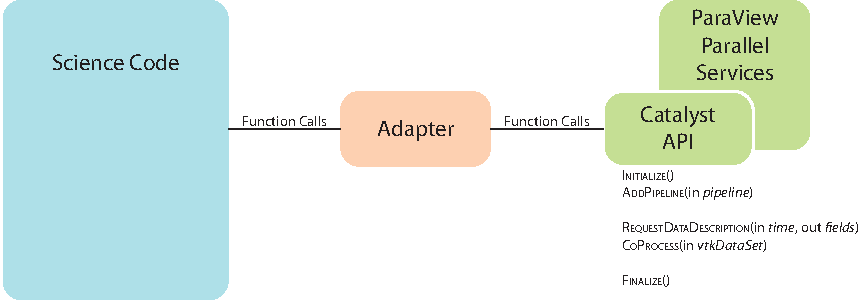
\includegraphics{figures/CatalystCoupling}
  \caption{Coupling a simulation with Catalyst.}
  \label{fig:CatalystCoupling}
\end{figure}

\subsection{Catalyst Architecture}

Catalyst boils the ParaView and VTK architecture down into five API calls that
manage all the processing required for operating a processing pipeline.
Initialize and Finalize are expected calls when dealing with MPI; this is where
Catalyst will first access MPI World.  RequestDataDescription and CoProcess
handle the hand-shake from the simulation code to Catalyst.
RequestDataDescription passed current time information to Catalyst, and
Catalyst passes back whether or not it should process and which fields it
needs.  This may allow the simulation code, through the adaptor described
below, to efficiently pass only what is necessary at that time.  The CoProcess
call is where control is passed to Catalyst for processing.  This call will
hang until Catalyst finishes and returns control to the simulation.

The AddPipeline call is where a majority of the work is done.  Although there
is usually only one pipeline added to Catalyst, it is possible to add several.
It is also common for this pipeline to be written in Python, because this is
the native scripting language for ParaView.  It is also possible for the
pipeline to be coded in C++.  While there is overhead cost to using
Python code in the pipeline here, it is very low due to its nature as a glue
code combining the C++ filters which are written in VTK.  The advantage to
using Python is that a scripted pipeline can change alongside the simulation
input deck without needing to recompile.

\begin{figure}[htb]
  \centering
  \includegraphics{figures/ScriptExport}
  \caption{Wizard plugin within ParaView to export interactive traces as 
Catalyst pipelines for use within a coupled simulation.}
  \label{fig:ScriptExport}
\end{figure}

In addition to the advantages of writing Python pipeline scripts by hand, there
is a well supported plugin for ParaView that will automatically create Catalyst
Python scripts automatically from within the GUI, based on what the user
does interactively, as shown in Figure~\ref{fig:ScriptExport}.  This plugin 
reads in a file and creates the same code 
object provided by the adaptor (see Section~\ref{sec:Adaptor}).  The rest of the
pipeline operates identically whether the data has been read in from a file
or it is coming from an in-memory \insitu transfer.  

The plugin creates images for each view open at the time the script is 
exported. 
To write files, one can create objects
within the pipeline that act as file write points.  In general, these are 
placed
at the end of a long chain of processing to store the resulting processed data,
but it is also possible to splice these file writes into in the pipeline at
any point, so that intermediate data can be preserved. 
Each file and image writer
can write at an independent frequency, so that the output can be tuned 
precisely by the analyst.  For example, images (which tend to be very small) 
can be written out frequently, while large, detailed data files can be written out 
infrequently.

\subsection{Simulation Adaptor}\label{sec:Adaptor}

Since Catalyst will extend to a variety of existing simulation codes, our
design does not expect its API to easily and efficiently process internal
structures in all possible codes directly.  Our solution is to rely on
adapters --- which are small pieces of code written for each new linked
simulation --- to translate data structures between the simulation's code
(for our use case the CTH shock physics code) and Catalyst's VTK-based
architecture, as shown in Figure~\ref{fig:CatalystCoupling}.  The adapter
must also establish a mechanism that allows the simulation to define a
visualization pipeline and periodically invoke the data analysis while running
the simulation, which in our CTH adapter we control through the CTH input
deck.

To conserve memory, our adapter directly interfaces the \vda code to the
data structures defined by CTH.  This interface is challenging because
although the blocks of data are represented sequentially in both CTH and
VTK, the multidimensional order is different.  To address this, our adapter
contains an interface wrapper above the standard VTK array.  The wrapper
reimplements the array's accessor functions to handle the order difference
between the two systems.  Although there is a minor overhead in additional
pointer arithmetic and virtual method calls, it saves us from a deep memory
copy.

\subsection{References}

The Catalyst library and the algorithms we use within CTH are an
accumulation of several years work, starting with the development of
fragment analysis algorithms with our post-processing
tools\lcite{Moreland2008:UltraVis,Ice2009,Moreland2010}, described in more
detail in Section~\ref{sec:UseCase}.  Subsequent work lead to the
development of Catalyst\lcite{Fabian2011} and the scaling of algorithms
used in conjunction with CTH\lcite{Fabian2012}.


\section{Nessie}
\label{sec:Nessie}

The NEtwork Scalable Service Interface, or Nessie, is a framework for developing
parallel client-server data services for large-scale HPC
systems~\cite{lofstead:2011:nessie-staging,oldfield:lwfs-data-movement,oldfield:2012:uGNI}. 

Nessie was originally developed out of necessity for the Lightweight File
Systems (LWFS) project~\cite{oldfield:lwfs}, a joint effort between researchers
at Sandia National Laboratories and the University of New Mexico. The LWFS
project followed the basic philosophy of ``simplicity enables scalability'',
the foundation of earlier work on lightweight operating system kernels at
Sandia~\cite{riesen:ccpe-lwk}. The LWFS approach was to provide a core set of
fundamental capabilities for security, data movement, and storage and afford
extensibility through the development of additional services. For example,
systems that require data consistency and persistence might create services for
transactional semantics and naming to satisfy these requirements. The Nessie
framework was designed to be the vehicle to enable the rapid development and 
deployment of such services.  


Although Nessie was originally designed for I/O and system services, it is also
useful for development of application-specific data services.  For example, 
we developed services for staging checkpoint
data~\cite{oldfield:ft-ldrd-tr,reiss:checkpoint-proxy,oldfield:modeling_checkpoints},
HPC database integration~\cite{oldfield:sql-proxy}, interactive
visualization~\cite{oldfield:multilingual-siam}, network traffic analysis, and 
most recently CTH in-transit analysis~\cite{moreland:2011:in-transit}.  A recent
paper describes these services in detail~\cite{lofstead:2013:data-staging}.


This section includes a brief description of the Nessie architecture and APIs followed
by a more detailed description of the in-transit service for CTH analysis using 
ParaView.  


\subsection{Nessie Architecture}

Because Nessie was originally designed for I/O systems, it includes a number of
features that address scalability, efficient data movement, and support for
heterogeneous architectures. Features of particular note include 1)~using
asynchronous methods for most of the interface to prevent client blocking while
the service processes a request; 2)~using a server-directed approach to
efficiently manage network bandwidth between the client and servers; 3)~using
separate channels for control and data traffic; and 4)~using XDR encoding for
the control messages (i.e., requests and results) to support heterogeneous
systems of compute and service nodes.

A Nessie service consists of one or more processes that execute as a serial
or parallel job on the compute nodes or service nodes of an HPC system. We have
demonstrated Nessie services on the Cray XT and XE systems at Sandia National
Laboratories (SNL) and Oak Ridge National , the Cray XT4/5 systems at Oak Ridge National Laboratory,
and a large InfiniBand
cluster at SNL. The Nessie RPC layer has direct support of Cray's SeaStar
interconnect~\cite{brightwell:2006:seastar}, through the Portals
API~\cite{brightwell:2002:portals3}; Cray's Gemini
interconnect~\cite{alverson:2010:gemini}; and
InfiniBand~\cite{infiniband:specification}.  

\subsubsection{Nessie API}

The Nessie API follows a remote procedure call (RPC) model, where the client
(i.e., the scientific application) tells the server(s) to execute a function on
its behalf.  Nessie relies on client and server stub functions to encode/decode
(i.e., marshal) procedure call parameters to/from a machine-independent format.
This approach is portable because it allows access to services on heterogeneous
systems, but it is not efficient for I/O requests that contain raw buffers that
do not need encoding. It also employs a `push' model for data transport that
puts tremendous stress on servers when the requests are large and unexpected,
as is the case for most I/O requests.


To address the issue of efficient transport for bulk data, Nessie uses separate
communication channels for control and data messages. In this model, a ``control''
message, also known as a request, is typically small. It identifies the
operation to perform, where to get arguments, the structure of the arguments,
and perhaps the data itself (if the data is small enough to fit in the
fixed-sized request).  In contrast, a data message is typically large and
consists of ``raw'' bytes that, in most cases, do not need to be
encoded/decoded by the server. For example,
Figure~\ref{fig:nssi-movement-protocol} shows the transport protocol for an
in-transit service that performs analysis of simulation data.

\begin{figure}
\begin{centering}
\includegraphics[scale=0.6]{figures/ServerDirected}
\caption[Nessie transport protocol]{Conceptual protocol for Nessie service doing analysis.  
The server fetches bulk data through
RDMA commands until it has satisfied the request.  After completing the
data transfers, the server processes the data, writes analysis results
to disk, then sends a small ``result'' back to the client
indicating success or failure of the operation.}
\label{fig:nssi-movement-protocol}
\end{centering}
\end{figure}

The Nessie client uses the RPC-like interface to push control messages to the
servers, but the Nessie server uses a different, one-sided API to push or pull
data to/from the client. This protocol allows interactions with heterogeneous
servers and benefits from allowing the server to control the transport of
bulk data~\cite{kotz:bdiskdir,seamons:panda}. The server can thus manage large
volumes of requests with minimal resource requirements. Furthermore, since
servers are expected to be a critical bottleneck in the system, a server
directed approach affords the server optimizing request processing for
efficient use of underlying network and storage devices -- for example,
re-ordering requests to a storage device~\cite{kotz:bdiskdir}.

While it is not strictly necessary on systems that have homogenous clients and servers, we 
use XDR encoding to provide portable serialization of arguments for the request arguments. 
This was a design decision made early in the project that allow the client to
send arbitrary C-like data structures to the server with minimal development effort.  At 
the time, we were implementing file services for a system where the service nodes were
a different architecture (and had different endienness) than the compute nodes.  In this 
case, byte-swaps were necessary for the control structures.  Since
\emph{rpcgen}, the function that generates the serialization code is pervasive in Unix
environments and has been in use for more than a decade, it was the logical choice for 
argument marshaling.  

\subsubsection{NNTI API}

The Nessie Network Transport Interface (NNTI) provides a portable, lightweight,
interface for RDMA operations on the major HPC platforms.  Our current
implementation includes support for the Cray Seastar, InfiniBand,
Cray Gemini, and IBM DCMF interconnects.  The APIs include commands
to open and close the interface, connect and disconnect to a peer,
register and deregister memory buffers, and finally asynchronously transport
(through put, get, and wait commands) bulk data. 

The NNTI library sits below the Nessie RPC library to enable portability across
HPC interconnects.  NNTI is also used by the
ADIOS/DataStager~\cite{abbasi:2010:datastager} to provide the same level of
portability and performance.

\subsubsection{CommSplitter API}

The CommSplitter library was designed to overcome a security model limitation in
the Gemini interconnect.  On current Gemini systems, user-space applications
are not allowed to communicate, even if both applications are owned by the same
user.  We requested this feature and at the time of this writing, Cray is
addressing this issue to better support data services in future versions of
Gemini.  In the mean time, we overcame that limitation by launching our jobs in
Multiple Program, Multiple Data (MPMD) mode.  MPMD mode enables a set of
applications to execute concurrently, sharing a single MPI Communicator.   The
problem with this approach is that legacy applications were not designed to
share a communicator with other applications.  In fact, most HPC codes assume
they have exclusive use of the \texttt{MPI\_COMM\_WORLD} communicator.  When
this is not the case, a global barrier, such as an \texttt{MPI\_Barrier}
function will hang because the other applications did not call the
\texttt{MPI\_Barrier} function. 

To address this issue, we developed the CommSplitter library to allow
applications to run in MPMD mode while still maintaining exclusive access to a 
virtual \texttt{MPI\_COMM\_WORLD} global communicator.  

The CommSplitter library identifies the processes that belong to each
application, then ``split'' the real \texttt{MPI\_COMM\_WORLD} into separate
communicators.   The library then uses the MPI profiling interface to intercept
MPI operations, enforcing the appropriate use of communicators for
collective operations.

No changes are required to the application source code to enable this
functionality.  The user simply links the CommSplitter library to the executable
before launching the job.  The library has no effect on applications that are
not run in MPMD mode. 



\subsection{CTH in-transit analysis}

In this milestone, we used Nessie to construct an in-transit CTH analysis 
service.  The analysis service exists as its own parallel job 
that communicates with a parallel CTH job using the Nessie APIs.  
The in-transit CTH analysis library is a drop-in replacement
for the PVSPY library~\cite{moreland:2010:coprocessing-milestone} used for
in-situ analysis.  This makes comparing in-situ and in-transit approaches
extremely convenient since it only requires the user to link a different
library when compiling CTH.  Instead of executing the analysis on the 
same compute nodes of the CTH application (as the in-situ library does), the
in-transit library marshals requests, sends data to the analysis service, and
performs all the analysis on the separate application.
Figure~\ref{fig:cth-service} illustrates this process for analysis that does
fragment detection. 

\begin{figure*}
\begin{centering}
\subfloat[In-situ analysis]{
  \includegraphics[scale=0.55]{figures/cth-in-situ}
  \label{fig:cth-in-situ}
}
\subfloat[In-transit analysis]{
  \includegraphics[scale=0.55]{figures/cth-in-transit}
  \label{fig:cth-in-transit}
}
\caption[In-Situ and In-Transit Analysis]{Comparison of in-situ (a) and in-transit (b)
fragment detection for the CTH shock physics code.}
\label{fig:cth-service}
\end{centering}
\end{figure*}

% There are a couple of trade-offs to consider when deciding whether to perform
% the analysis in-transit or in-situ.  First, the in-transit approach allows
% fragment detection to execute in parallel with CTH, unlike the in-situ approach
% that requires CTH to wait for the analysis to complete.  If the time to execute
% the analysis code is substantially larger than the time to transfer the raw data
% to the service, there is a performance advantage to using the in-transit
% approach.

% A second consideration is library scalability.  While significant effort has
% gone into making the CTH code scale to extremely large core counts, not as much
% effort has gone into scalability of the analysis code.  For example, the
% ParaView coProcessing libraries have not successfully run on more than 32
% thousand cores.  Linking CTH to ParaView for in-situ analysis also limits the
% scalability of the CTH run.  In contrast, the data service will likely use
% a much smaller number of cores, putting no limitation on the scale of CTH. 

% Another often overlooked consideration is the memory required to link a large
% analysis library into a production scientific code.  In the in-situ case, CTH
% has to link ParaView.  Since many HPC systems do not efficiently support dynamic
% libraries\footnote{Support for dynamic libraries is currently being evaluated
% for the Cray XE6.}, the entire static ParaView library has to be linked. On the
% Cray XE6, the in-situ binary for CTH is 330 MiB, where the in-transit binary for CTH is 30
% MiB.  That is a substantial difference, especially on systems that are memory
% limited -- as is the case for most multi-core HPC platforms.


For efficiency reasons, the in-transit PVSPY client implementation does not
simply forward all the functions to the service.  In many cases, the client
maintains metadata to avoid unnecessary data transfers.  For example, the PVSPY
API includes ``setup'' functions for initializing data structures, assigning
cell and material field names, and setting cell and material fields pointers.
Not all of these functions require an immediate interaction with the data
service.  In fact, the only operations that require bulk data transport are
the operations that synchronize the metadata and the data between the client 
and the server.  These operations occur just before a \emph{pvspy\_viz} operation
that initiates the ParaView coProcessing on the remote service. 

The in-situ version of PVSPY has the notion of a ``CTH source'' that allows the
analysis code to work directly on the memory of the CTH application without
making any copies.   Since the in-transit service does not have access to the
physical memory of the CTH application, we created a virtual CTH source on the
server that emulates the data structures on the CTH application.  That allows
the service to use use the same PVSPY library that the client uses in the in-situ
analysis.  

With the exception of the operations to transfer metadata and data to the analysis
service, all remote operations are asynchronous, allowing the analysis on the 
service to execute in parallel with computation on the CTH application.  If one
remote visualization operation is not complete by the time CTH is ready to do another
visualization operation, CTH has to wait. 


\subsection{Related Efforts}

There are a number of efforts to develop technologies for staging data or 
providing data services that are related to, and in some cases derived from,
Nessie.  The two primary competitors of Nessie include the data-staging
portions of the ADIOS library from ORNL, and the Glean library from Argonne
National Laboratory. 

The Adaptable IO System (Adios) is an I/O library that separates the I/O
interface from the underlying I/O operations.  Using XML configuration 
files, the user can specify, at runtime, the methods used to perform I/O.
For example, MPI-IO, POSIX-IO, netCDF, or their own BP method are all options
the use can select.  ADIOS also includes methods data transport that allow
the staging and processing of data in the same way as Nessie.  This staging
technology, called DataTap~\cite{datatap2009cluster} and
DataStager~\cite{abbasi:2010:datastager} derive from early work on Nessie as
part of a joint collaboration between GA Tech, SNL, and ORNL.  More recent
versions of DataStager are also using the NNTI API to provide portable 
RDMA transport. 

The DataSpaces~\cite{docan:2010:dataspaces} project uses the memory on
data-staging nodes as a scratch space for communicating and sharing 
data among multiple applications.  This work is closely aligned with the 
ADOIS efforts at ORNL.  The primary focus is to use asynchronous IO to
move data into a staging area and then having a
different application retrieve data at a later time.

A recent effort called Glean~\cite{vishwanath:2011:glean} from Argonne is a
start towards both accelerating IO performance and integrating functionality,
such as analysis routines, at the right place transparently. It is very similar
to PreDatA, but extends the location of operations to potentially beyond the
current machine.

Most of the related efforts focus primarily on the I/O benefits of data-staging, but
have not put a tremendous effort into complex analysis. The majority of the analyis
codes relatively simple statistics and visualization.  With Nessie, and 
this effort in particular, we treat the service as a potentially complext parallel application
that includes all the synchronization, communication, and scaling issues inherent in HPC 
parallel applications.  These issues require a level of detail and performance 
tuning that is lacking in other efforts.  

A second distinction between our approach and related work is a general 
philosophy on supporting APIs.  While the other approaches, like ADIOS,
provide a unified I/O API, our approach is to provide in-transit
implementations of commonly used APIs so the code does not have to change the
source code.  It was this approach that made comparison between the in-situ and
in-transit approaches so easy to perform.

\subsection{Nessie Availability}

The Nessie software is available, open source, as part
of the Trilinos I/O Support Package~\cite{oldfield:2012:trios-journal}.
The package includes the NNTI, Nessie, CommSplitter libraries as well
as a collection of CMake macros and other tools for constructing 
applicatio-specific data services for a variety of different HPC 
platforms. 




\section{Use Case}
\label{sec:UseCase}

\fix{Nathan}

\fix{Description of problem.}

\fix{Description of algorithms.}


\section{Results}
\label{sec:Results}

\fix{Nathan and Ron}

\begin{figure}[htb]
  \centering
  \includegraphics[width=\linewidth]{figures/MemoryUsagePerNode.pdf}
  \caption{Plot of average per node memory usage of the run on Cielo.}
  \label{fig:MemoryPerNode}
\end{figure}

\begin{figure}[htb]
  \centering
  \includegraphics[width=\linewidth]{figures/MemoryUsageTotal.pdf}
  \caption{Plot of average total memory usage of the run on Cielo.}
  \label{fig:MemoryTotal}
\end{figure}


\section{Conclusions}
\label{sec:Conclusion}

This document summarizes a significant scaling study resulting from over 9
million core-hours of execution and analyzes the comparative performance of
multiple workflows for performing \vda on simulation results.  Most of
these workflows benefit from running in tandem with the simulation to
analyze its transient data before it is written to storage.  Based on this
analysis, we make the following conclusions.

\paragraph{\Intransit can provide a performance improvement over \insitu in
  some circumstances, but the window is more narrow than we initially
  thought.}  \Intransit analysis has an added overhead above embedded
\insitu analysis involving transferring data between parallel jobs.  Given
an analysis with perfect linear scalability, we suspect \intransit
workflows will always have an added cost, and our results support this.
With an analysis that does not scale perfectly, possibly due to
communication overhead, it is theoretically possible for \intransit to be
faster by reducing the size of the analysis job.  This is one of the
motivations for choosing an analysis task that requires significant
communication.  In our results, we do find instances where \intransit is
faster, but by a smaller margin and for fewer configurations than we
initially anticipated.  So although \intransit has several other positive
features, we do not anticipate performance to be the main motivations for
using it.

\paragraph{Memory overhead will be an important trade-off space.}
The baseline amount of memory added to the CTH job to perform \insitu
processing is roughly 100MB per core.  Considering that our embedded
\insitu library is a fully featured visualization toolkit containing over 2
million lines of code and algorithms developed over almost 2 decades, this
overhead is not unreasonable.  Nevertheless, this footprint can be
problematic for simulations already tight on memory.  Because of this,
efforts are already underway to improve our memory footprint by making
finer modules and being more selective on the available algorithms.  This,
of course, requires a compromise between the size of the library and the
algorithms that are dynamically available.  We also note that our algorithm
has the potential to generate sizable meshes of its own.  Thus, it may be
fruitful to pursue and support incremental algorithms where possible.

\paragraph{Initialization time matters.}  Our scaling efforts to date
focus on the scalability of the algorithms invoked during the run of a
simulation.  The initialization cost, a one-time penalty, has yet to be
seriously considered.  However, based on our HPCToolkit measurements,
initialization becomes a significant cost at high process counts.

\paragraph{Disk-based I/O is not dead\ldots{} yet.} Our initial assumption
was that it would not be feasible to output full results at a fine enough
temporal resolution from CTH to disk storage to perform our high fidelity
analysis.  However, our control workflow shows that although the overall
time to write data to disk and then read back again incurs a large cost, it
is still realistic to do so.  Thus, users may still choose to incur the
extra overhead to use a traditional offline post-processing \vda workflow.

\paragraph{Better job scheduling is important.} One of the more complicated
parts of running an \intransit workflow is scheduling the simulation job
and service job to run in tandem.  Frankly, the capabilities of the
scheduler are inadequate for our needs.  We cannot start and stop jobs
independently and make reconnections dynamically.  Another experiment we
would like to do but is challenging to schedule is to allow simulation and
service to share nodes.  Since each node has 16 cores, perhaps we could get
better transfer performance by allocating one core per node for service and
the rest for simulation.  A similar scheduling scheme will be important to
take advantage of burst buffers in future architectures.

\fix{Timeline of work ahead.}



% ---------------------------------------------------------------------- %
% References
%
\clearpage
% If hyperref is included, then \phantomsection is already defined.
% If not, we need to define it.
\providecommand*{\phantomsection}{}
\phantomsection
\addcontentsline{toc}{section}{References}
\bibliographystyle{plain}
\bibliography{MilestoneFY13,oldfield}


% ---------------------------------------------------------------------- %
%
\appendix

\section{Signed Letter from Committee}

\section{Executive Summary Slides}

\section{Raw Data}

% \printindex

%
% Some distributions are required by Sandia; e.g. the housekeeping copies.
% Depending on the type of report; e.g. CRADA, Patent Caution, etc.
% additional distribution lines may have to be added. See the "Guide for
% Preparing SAND Reports"
%
% SANDdistribution takes CA or NM as an optional argument. If given,
% the approrpiate housekeeping copies are inserted autmatically.
% Inside the SANDdistribution environment, several commands can be used
% insert the distributions for CRADA, LDRD, etc. See example below.
%
% You can leave the CA or NM option off and not use any of the SANDdist*
% commands. This will allow you to create a distribution list manually.
%
\begin{SANDdistribution}[NM]

  % Some external Addresses
  \SANDdistExternal{1}{James Ahrens\\ Los Alamos National Laboratory\\ P.O. Box 1663\\ Los Alamos, NM 87545}
  \SANDdistExternal{2}{David Rogers\\ Los Alamos National Laboratory\\ P.O. Box 1663\\ Los Alamos, NM 87545}
  \SANDdistExternal{1}{Berk Geveci\\ Kitware, Inc.\\ 28 Corporate Drive\\ Clifton Park, NY 12065}
  \SANDdistExternal{1}{Lucy Nowell\\ U.S. Department of Energy\\ SC-21\\ 19901 Germantown Road\\ Germantown, MD 20874-1290}
  \SANDdistExternal{1}{Becky Springmeyer\\ Lawrence Livermore National Laboratory MS 555\\ P.O Box 808\\ 7000 East Ave.\\ Livermore, CA 94551}

  \bigskip


  % Internal Addresses
  \SANDdistInternal{1}{1319}{Ronald Brightwell}{01423}
  \SANDdistInternal{1}{0845}{Micheal Glass}{01545}
  \SANDdistInternal{1}{1319}{Suzanne Kelly}{01423}
  \SANDdistInternal{1}{0845}{Kyran Mish}{01542}
  \SANDdistInternal{1}{0823}{Constantine Pavlakos}{09326}
  \SANDdistInternal{1}{0380}{Kendall Pierson}{01542}
  \SANDdistInternal{1}{0783}{Jason Wilke}{06615}

  \SANDdistInternal{2}{1326}{Nathan Fabian}{01461}
  \SANDdistInternal{2}{1326}{Kenneth Moreland}{01461}
  \SANDdistInternal{2}{1327}{Ron Oldfield}{01461}

  \SANDdistInternal{2}{0822}{Jeff Mauldin}{09326}
  \SANDdistInternal{2}{0822}{Warren Hunt}{09326}

\end{SANDdistribution}



% The second printing
%\begin{SANDreDistribution}
%    \SANDdistExternal{}{}
%    \bigskip
%    \SANDdistInternal{}{}{}{}
%    \SANDdistInternalM{}{}{}{}
%\end{SANDreDistribution}

\end{document}
